\interlude[2]<Trials \textasciitilde\ Attacks found>{ChronoTrigger}
\hypertarget{state-disruption}{%
\section{State Disruption}\label{state-disruption}}

\begin{frame}{In the following slides, you will learn…}
\hypertarget{you-will-learn-hybrid}{}
\begin{columns}[fullwidth]
  \begin{column}{.58\linewidth}
    …that denial of service can happen on the level of cryptography protocols!

    \vspace{2em}
    …that the wall clock is not to be trusted.

    \vspace{2em}
    …how to accept replay attacks and face them without fear!
  \end{column}
  \begin{column}{.20\linewidth}
    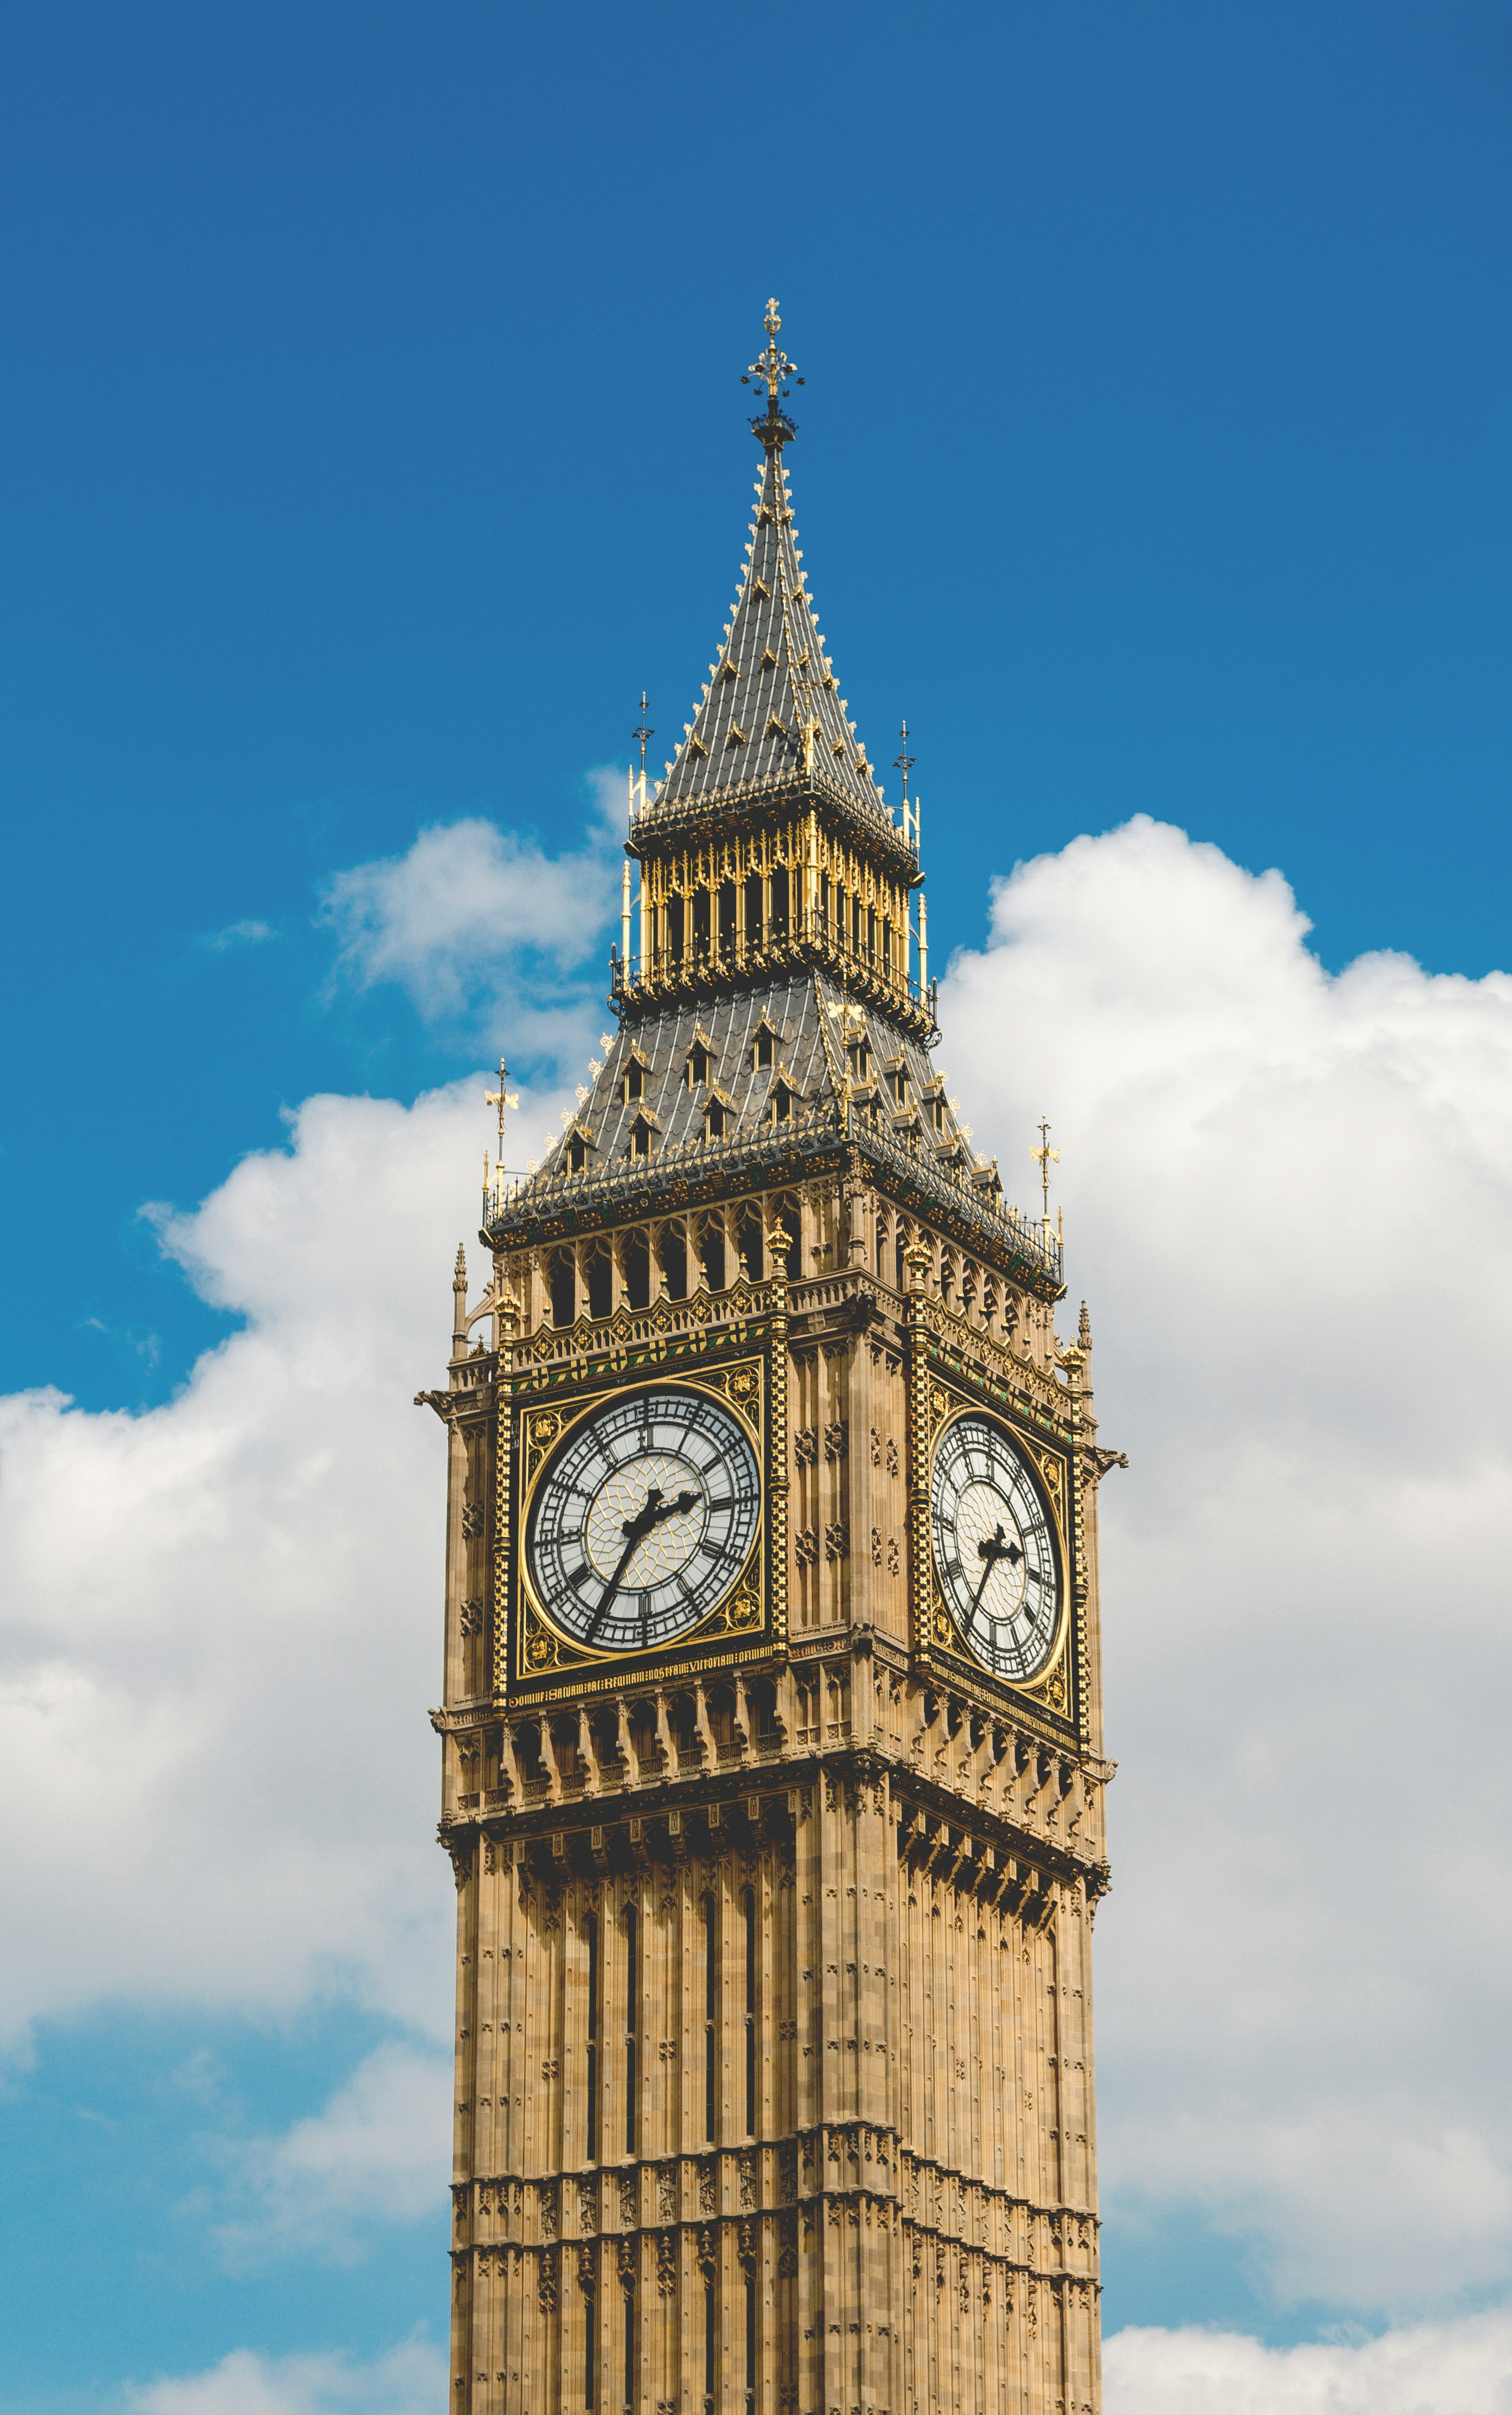
\includegraphics[width=\linewidth]{graphics/big-ben.jpg}
    \vspace{0.4cm}
  \end{column}
  \begin{column}{.20\linewidth}
    \vspace{1.6cm}
    \includegraphics[width=\linewidth]{graphics/sad-bunny-looking-left.jpg}
  \end{column}
\end{columns}
\end{frame}


\begin{frame}{What are State Disruption Attacks?}
  \raisebox{0pt}[0pt][0pt]{
    \begin{minipage}{\textwidth}
      \vspace{2.2cm}
      \begin{columns}[T,fullwidth]
        \begin{column}{.325\linewidth}
          \reflectbox{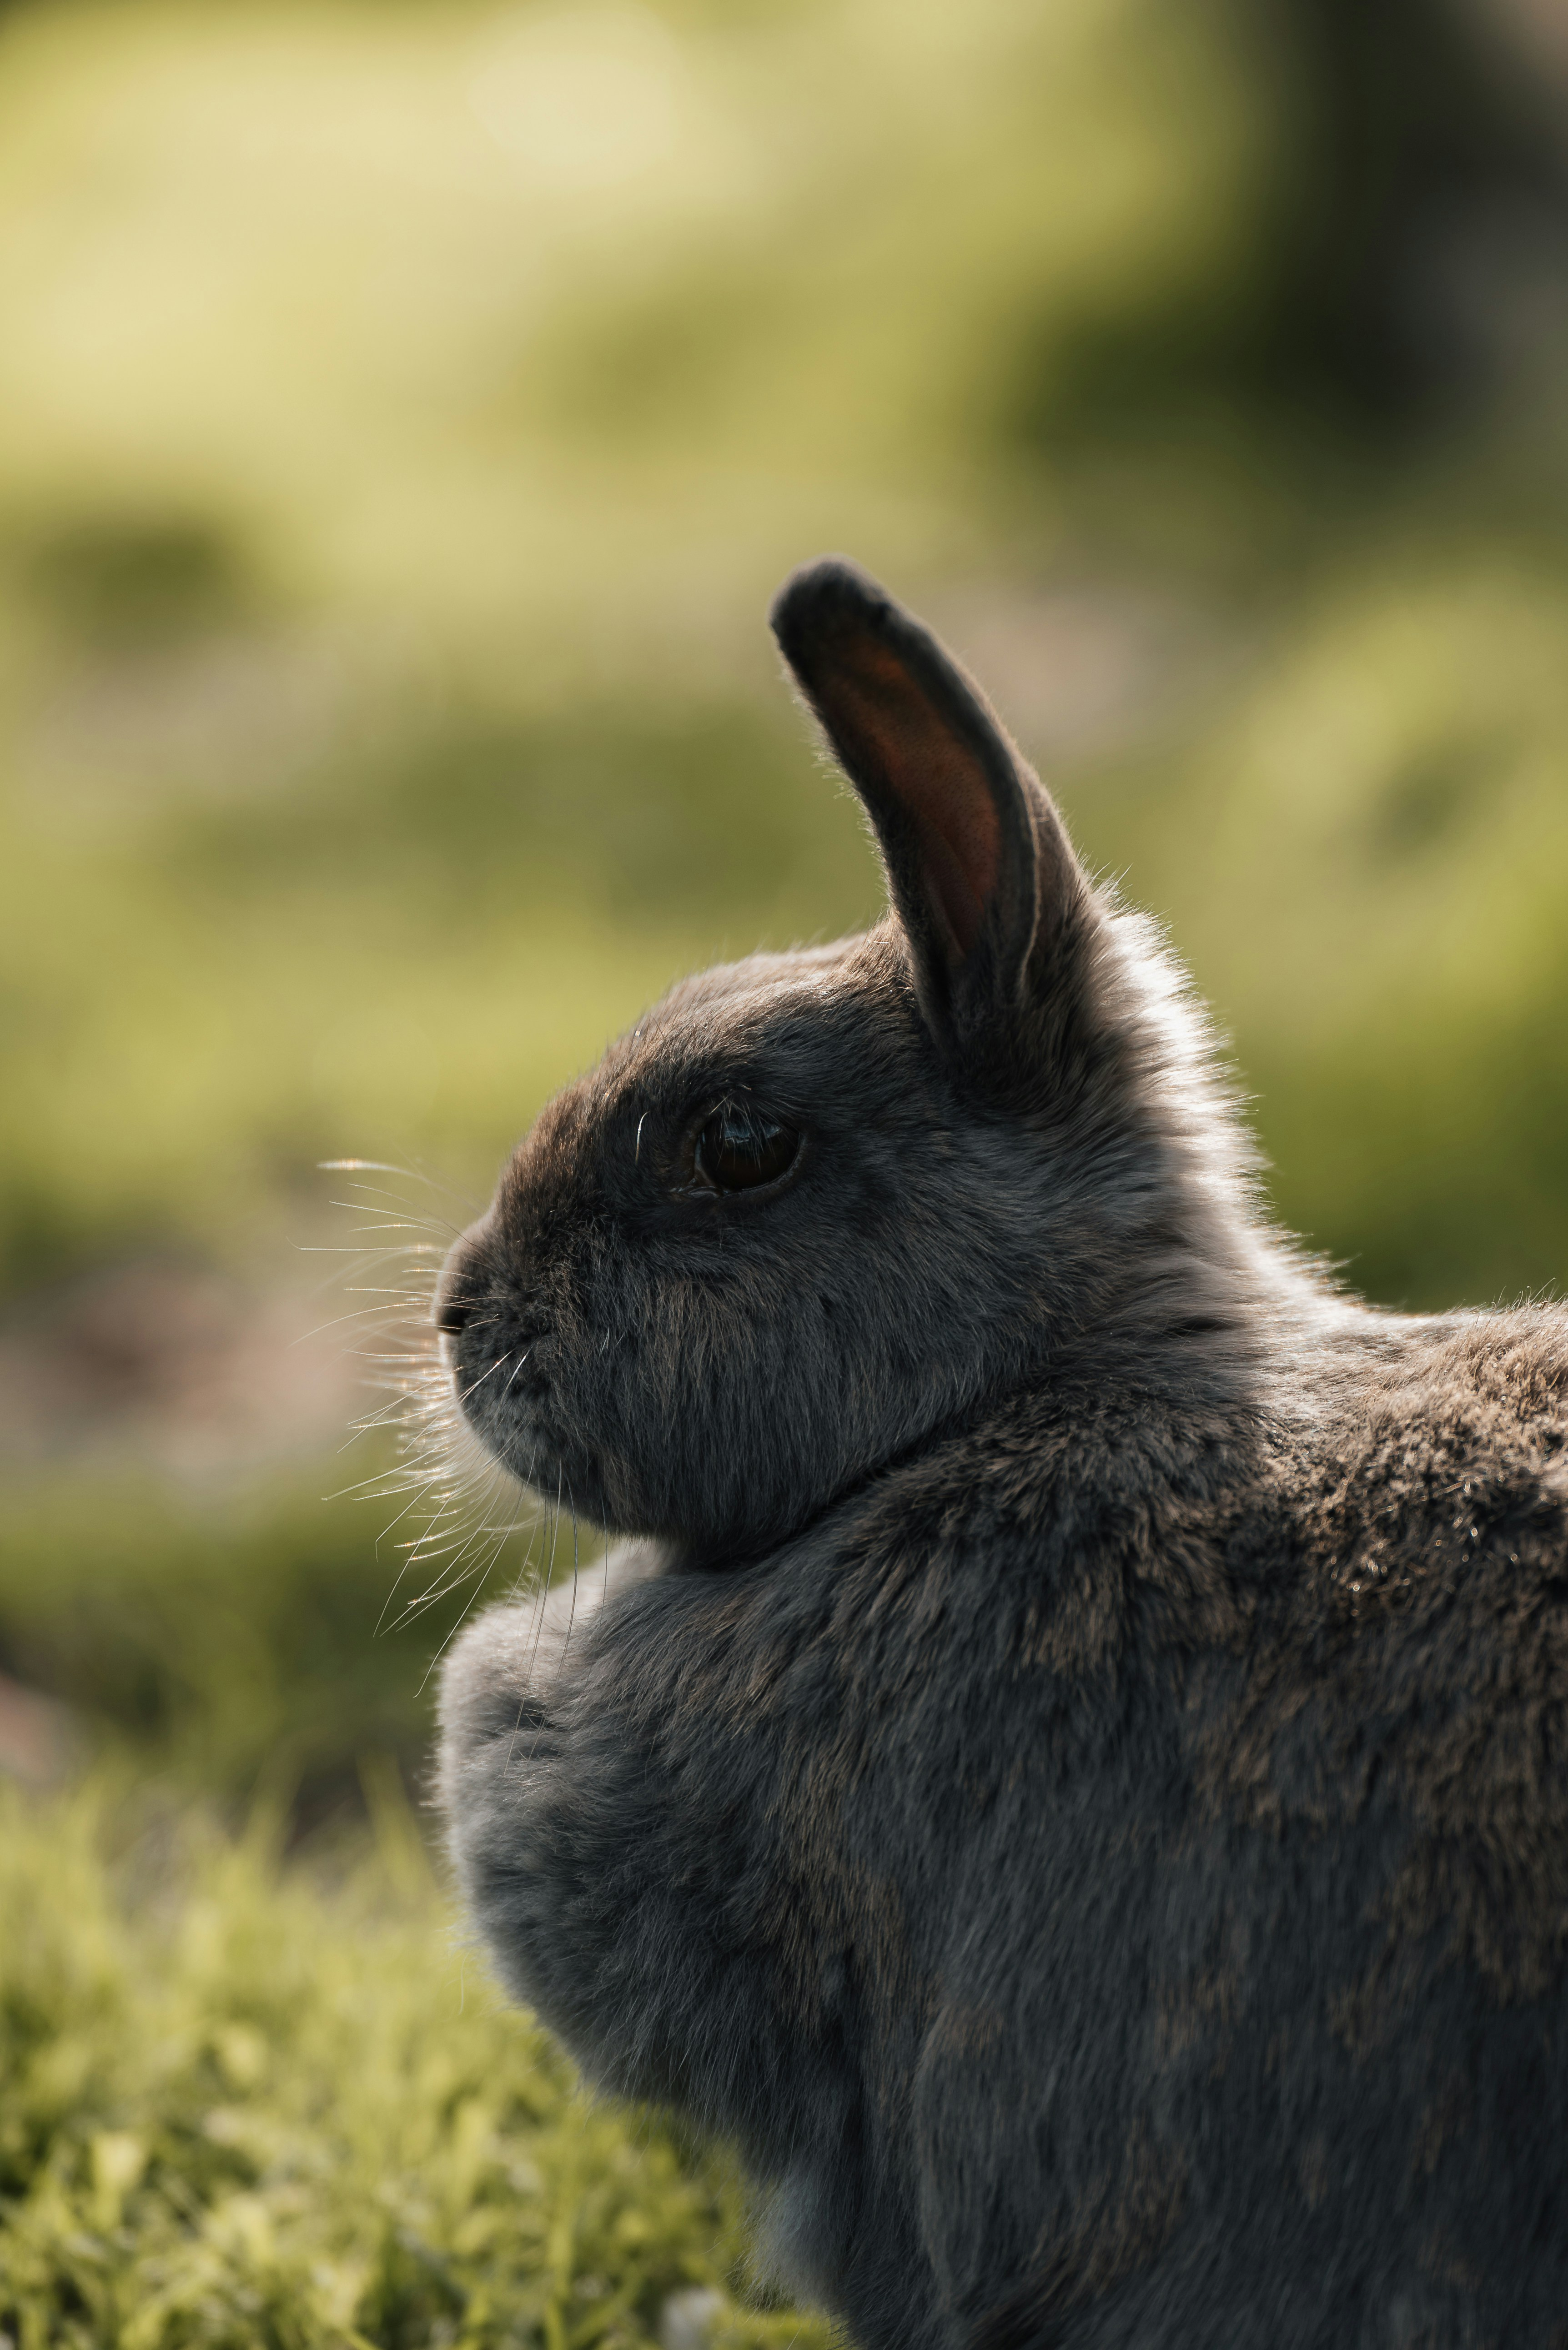
\includegraphics[width=0.9\linewidth,height=.454\textheight,padding=0cm 0cm .5cm 3cm,right,clip,trim={0cm 16cm 0cm 40cm}]{graphics/bunny-2.jpg}}
        \end{column}
        \begin{column}{.35\linewidth}
          \centering
          \includegraphics[width=0.9\linewidth,height=.85\textheight,trim={7cm 38cm 5cm 10cm},clip]{graphics/wires.jpg}
        \end{column}
        \begin{column}{.325\linewidth}
          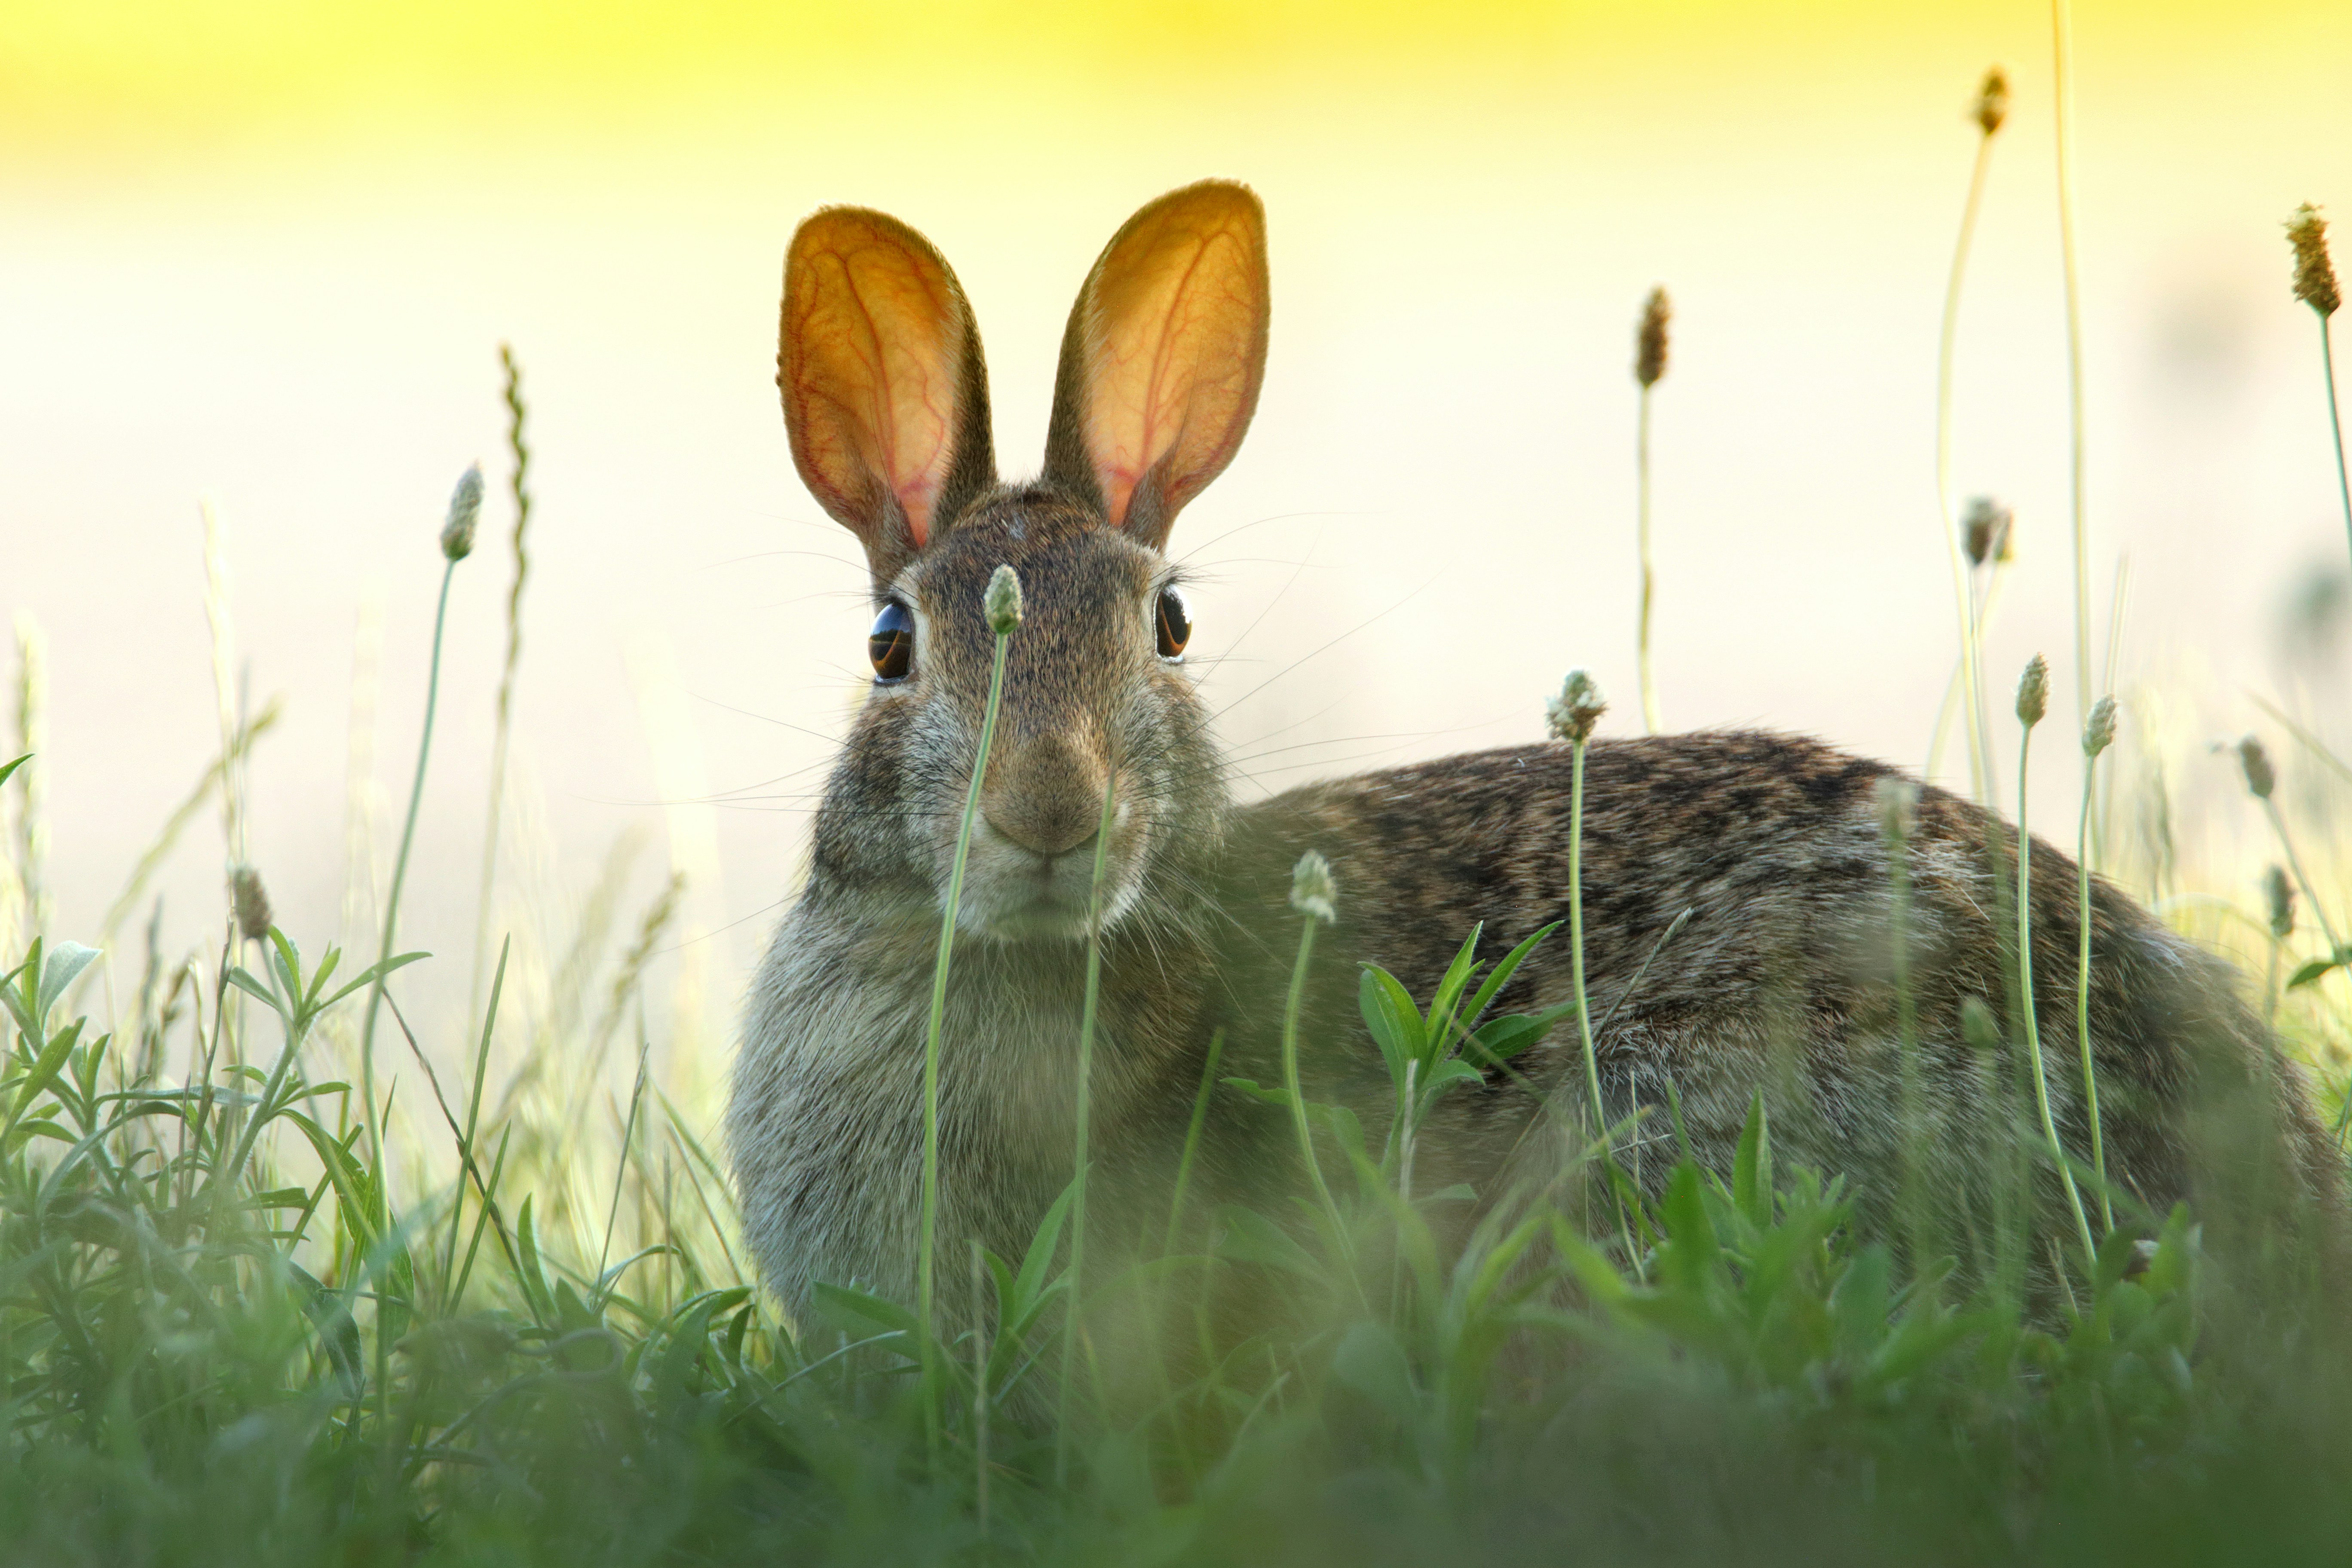
\includegraphics[width=0.9\linewidth,padding=0cm 0cm 0cm 0cm]{graphics/bunny-3.jpg}
        \end{column}
      \end{columns}
    \end{minipage}
  }
  \raisebox{0pt}[0pt][0pt]{
    \begin{minipage}{\textwidth}
      \centering
      \vspace{0.7cm}
      \hspace{1.3cm}\tikz\node[rectangle,fill opacity=1,fill=white,minimum height=4em, text width=0.38\linewidth]{
        \Large
        \hspace{0.1cm}Protocol level DOS
      };
    \end{minipage}
  }

  % \begin{itemize}
  %   \item Attacker trying to perform a protocol-level DOS attack
  %   \item Attacker may observe messages
  %   \item Attacker may insert messages, but they may not drop or modify messages
  %   \item Halfway between an active and passive attacker:
  %   \begin{itemize}
  %   \item For a fully active attacker state disruption is trivial; they can just drop messages
  %   \end{itemize}
  % \end{itemize}
\end{frame}




\begin{frame}{Retransmission Protection in WireGuard}
\hypertarget{retransmission-protection-in-wireguard}{}
\begin{columns}[fullwidth,T]

  \begin{column}{.5\linewidth}
    \vspace{-0.2cm}
    \rlap{\includegraphics[width=1.08\linewidth,page=3,clip=true,trim=0cm 2cm 0cm 1.9cm]{graphics/rosenpass-attack-types.pdf}}
  \end{column}

  \begin{column}{.46\linewidth}
    \vspace{0.4cm} % Manual alignment with blue box in graphic
    \begin{itemize}
      \item Replay attacks thwarted by counter
      \item Counter is based on real-time clock
      \item Responder is semi-stateful (one retransmission at program start may be accepted, but this does not affect protocol security)
      \item[$\Rightarrow$]
         WG requires \emph{either} reliable real-time clock \emph{or} stateful initiator
      \item[$\Rightarrow$]
        Adversary can attempt replay, but this cannot interrupt a valid handshake by the initiator
      \item[!] Assumption of reliable system time is invalid in practice!
    \end{itemize}
  \end{column}
\end{columns}
\end{frame}




\begin{frame}{ChronoTrigger Attack}
\begin{columns}[fullwidth,T]
  \begin{column}{.5\linewidth}
    \vspace{-0.2cm}
    \rlap{\includegraphics[width=1.08\linewidth,page=5,clip=true,trim=0cm 2cm 0cm 1.9cm]{graphics/rosenpass-attack-types.pdf}}
  \end{column}

  \begin{column}{.46\linewidth}
    \small\leavevmode
    \only<+|handout:+>{
      \begin{enumblock}{Preparation phase:}
      \begin{enumerate}
        \item \textbf{Attacker} sets \emph{initiator system time} to a future value
        \item \textbf{Attacker} records \emph{InitHello} as \emph{KillToken} while both peers are performing a valid handshake
      \end{enumerate}
      \end{enumblock}
\centerline{ \small … both peers are being reset … }
      \begin{enumblock}{Delayed execution phase:}
      \begin{enumerate}
        \item \textbf{Attacker} sends \emph{KillToken} to responder, setting their timestamp to a future value
        \item[$\Rightarrow$] Initiation now fails again due to timestamp mismatch
      \end{enumerate}
      \end{enumblock}
    }

    \only<+|handout:+>{%
      \begin{block}{Gaining access to system time:}
      \begin{itemize}
        \item Network Time Protocol is insecure,\\
        Mitigations are of limited use
        \item[$\Rightarrow$] Break NTP \emph{once}; kill token lasts forever
      \end{itemize}
      \unskip
      \end{block}
    }

    \only<+|handout:+>{%
      \leavevmode\begin{block}{Attacker gains}
      \begin{itemize}
        \item Extremely cheap protocol-level DOS
      \end{itemize}
      \unskip
      \end{block}

      \begin{block}{Preparation phase, attacker needs:}
      \begin{itemize}
        \item Eavesdropping of initiator packets
        \item Access to system time
      \end{itemize}
      \unskip
      \end{block}

      \begin{block}{Delayed execution, attacker needs:}
      \begin{itemize}
        \item No access beyond message transmission to responder
      \end{itemize}
      \unskip
      \end{block}
  }
  \end{column}
\end{columns}
\end{frame}




\begin{frame}{ChronoTrigger: Changes in Rosenpass}
  \begin{columns}[fullwidth,c]

    \begin{column}{.2\linewidth}
      \vspace{-0.2cm}
      \rlap{\includegraphics[height=\textheight,page=7,clip=true,trim=0.5cm 0.1cm 13cm 3cm]{graphics/rosenpass-attack-types.pdf}}
    \end{column}

    \begin{column}{.2\linewidth}
      \vspace{-0.2cm}
      \rlap{\includegraphics[height=\textheight,page=7,clip=true,trim=13cm 0.1cm 0.5cm 3cm]{graphics/rosenpass-attack-types.pdf}}
    \end{column}

    \begin{column}{.56\linewidth}
      \begin{itemize}
        \item InitHello is unauthenticated because responder still needs to encapsulate secret with initiator key
        \item Since InitHello is unauthenticated, retransmission protection is impossible
        \item Responder state is moved into a cookie called \emph{Biscuit}; this renders the responder stateless
        \item Retransmission of InitHello is now easily possible, but does not lead to a state disruption attack
        \item[$\Rightarrow$] Stateless responder prevents ChronoTrigger attack
      \end{itemize}
    \end{column}
  \end{columns}
\end{frame}




\begin{frame}{Rosenpass Key Derivation Chain: Spot the Biscuit}
  \hypertarget{rosenpass-kdf-chain-spot-the-biscuit}{}
  \centering
  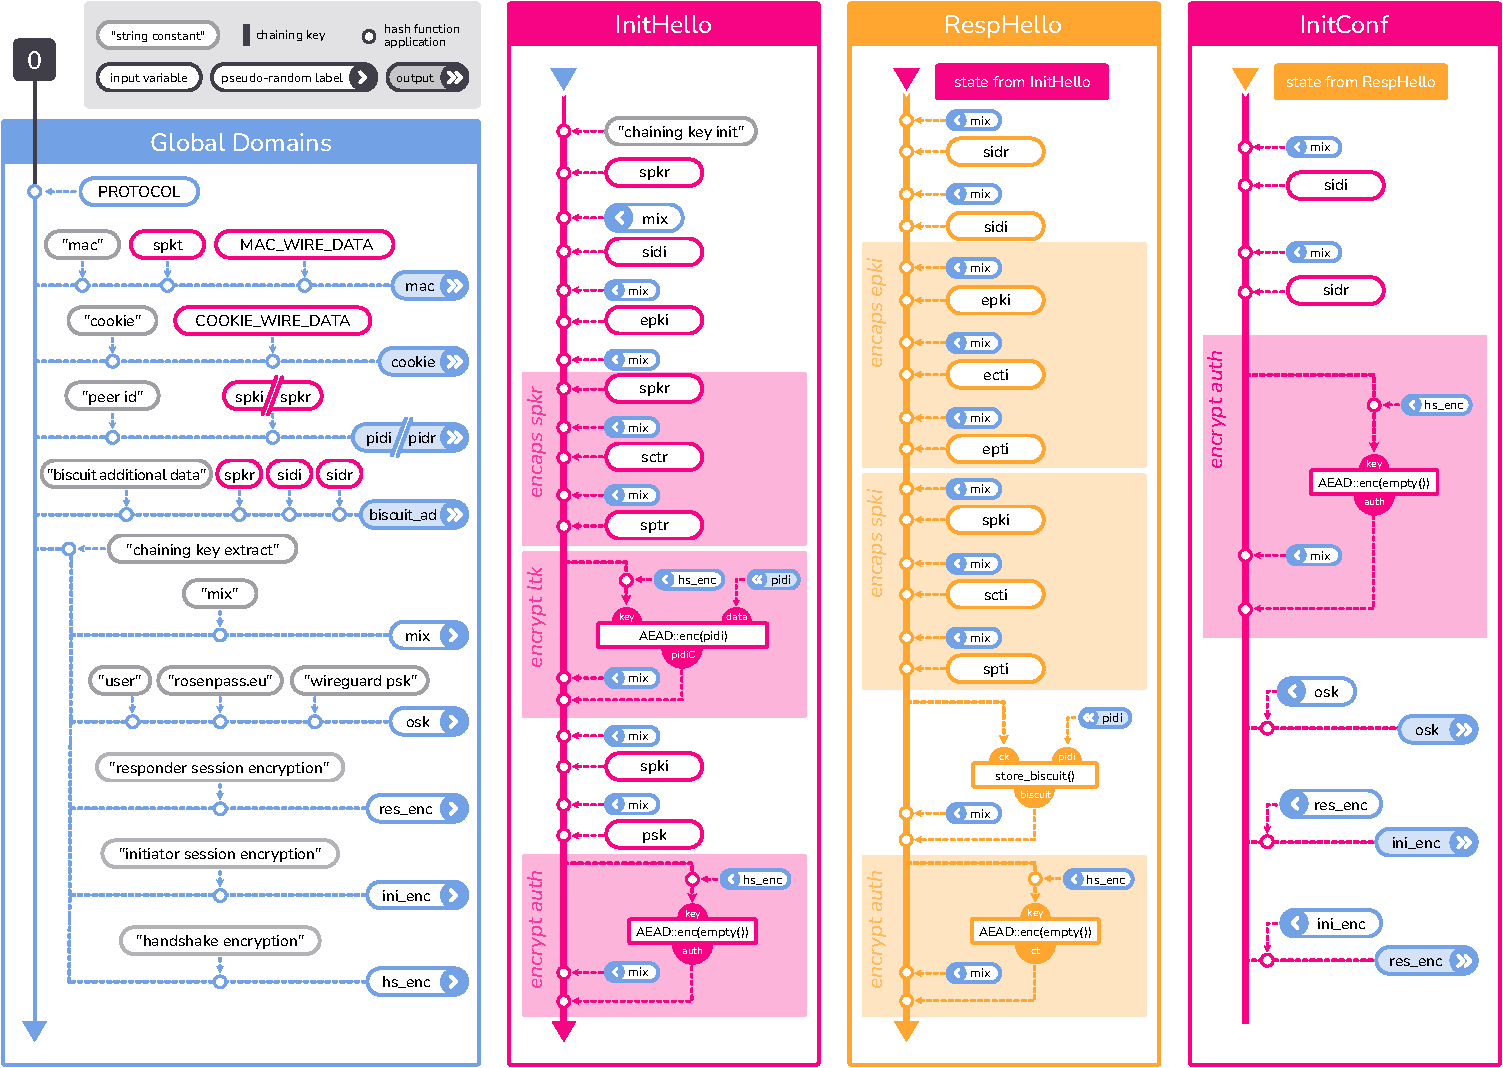
\includegraphics[height=.85\textheight]{graphics/rosenpass-wp-hashing-tree-rgb.pdf}
\end{frame}




\begin{frame}{Rosenpass Protocol Messages: Spot the Biscuit}
  \hypertarget{rosenpass-protocol-messages-spot-the-biscuit}{}
    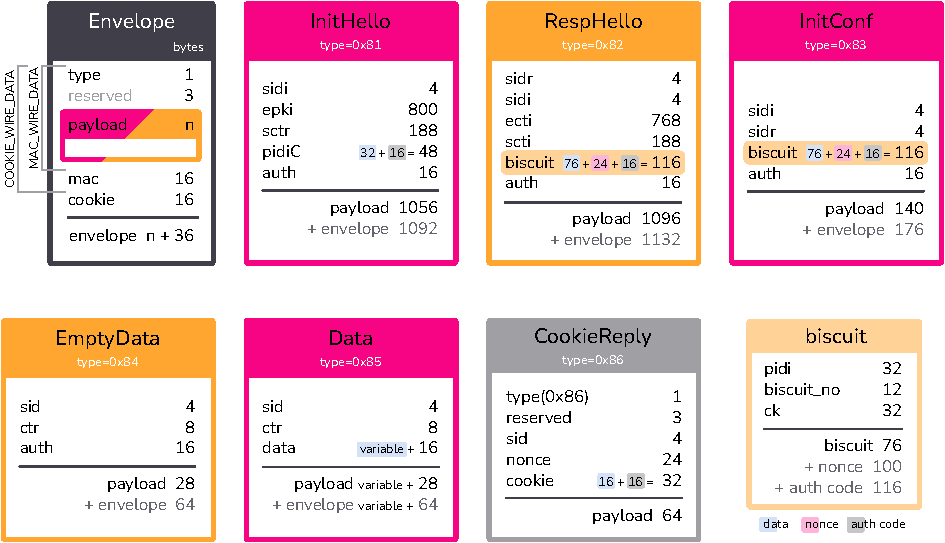
\includegraphics[height=.85\textheight]{graphics/rp-messages-04-all-rgb.pdf}
\end{frame}
